\chapter{Понятие цифровых моделей рельефа и их классификация}

Цифровая модель рельефа представляет собой поверхность местности, которая не включает в себя объекты, находящиеся на поверхности, которая создается на основе данных о высоте. Поверхность местности может быть представлена как трехмерная (3D) или двумерная (2D) \cite {1, 23}.

Источники для исходных данных для построения ЦМР очень разнообразны: 

\begin{enumerate} 
  \item[1)] радарная топографическая съемка местности;
  \item[2)] методы кинематической глобальной навигационной спутниковой системы;
  \item[3)] данные дистанционного зондирования Земли;
  \item[4)] материалы полевых съемок;
  \item[5)] методы определения структуры по движению;
  \item[6)] интерполяция цифровых контурных карт или данных из прямых съемок поверхности земли и другие \cite{2, 17}.
\end{enumerate}

При помощи ЦМР можно извлекать различные данные, например, зернистость и шероховатость поверхности, различные уклоны и изломы, также параметры, которые связаны с гидрографическими сетями. 

С помощью ЦМР можно автоматически извлечь морфометрические данные, такие как уклоны и изломы, аспект уклона, альтиметрические пояса, шероховатость или зернистость поверхности, а также параметры, касающиеся гидрографических сетей. Также при использовании ЦМР можно решить задачи связанные с оценкой форм склонов, через кривизну их поперечного сечения, проведением интерполяции по значениям высот, проведением трехмерной визуализации рельефа, проведением оценки видимости или невидимости  с определенной точки обзора и многие другие \cite{15,13}.

Существуют определенные требования, которым цифровая модель рельефа должна соответствовать:

\begin{enumerate} 
  \item[1)] модель должна содержать в себе доступную информацию, которую получают в результате наблюдений;
  \item[2)] параметры, которые присущи модели, должны иметь однозначный физический смысл и возможность прямого измерения;
  \item[3)] систематизация значений параметров позволит использовать их при моделировании стока в малоизученных бассейнах \cite{3,21}.
\end{enumerate} 

Также модель рельефа может быть представленна как матрица высот или матрица качеств.
\section{Матрицы высот рельефа местности}

Матрица высот может быть построена по тем данным объектов карты рельефа местности, которые имеют абсолютную высоту или 3D-метрику. В задачах анализа рельефа, которых касаются построения профилей и зон видимости, а также в задачах вычисления площади или длины объекта с учетом рельефа такая матрица высот может использоваться в качестве основы. Также в задачах моделирования зон затопления, формирования объемной карты местности, определения направления склонов и других \cite{4,12}.

Для формирования трехмерной метрики определенных объектов, содержащихся на карте, или для получения отмывки рельефа в виде растрового изображения, оценки и анализа статистики поверхности указанного участка местности, а также для создания автоматического построения изолиний -- используют матрицу высот рельефа \cite{5,14}. Пример матрицы высот изображен на рисунке   \ref{fig:1}.
\begin{figure}[h!]
    \center
    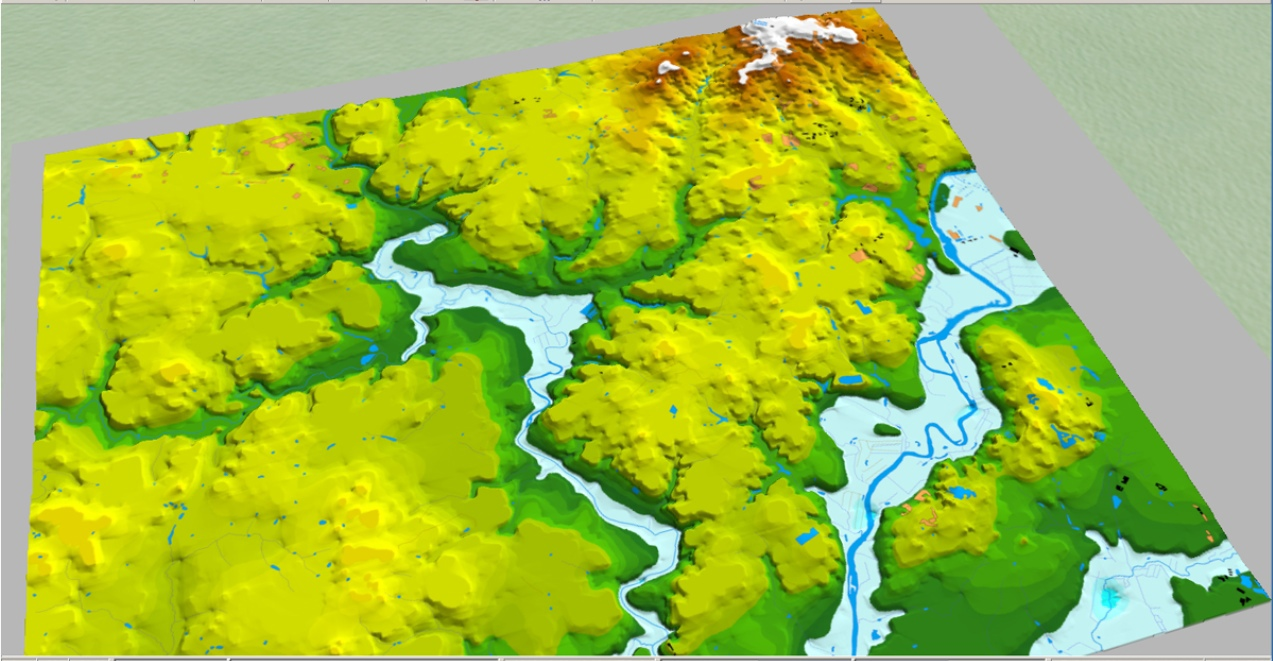
\includegraphics[scale=0.3]{images/112.jpg}
    \caption{Пример матрицы высот}
    \label{fig:1}
\end{figure}

\section{Использование матриц качеств для характеристик поверхности}

Обычно матрицу качеств представляют в виде поверхности значений определенной моделируемой характеристики. Для построения матрицы качеств могут использоваться значения смысловой характеристики объектов, содержащиеся на векторной карте или в выбранных полях таблицы базы данных \cite{6, 7}. 

Данные, которые может содержать матрица качеств очень различны. Это может быть, как тип растительности или землевладения, плотность застройки, так и качественные характеристики почвы, глубина залегания грунтовых вод, концентрация выхлопных газов и т.д.

Модель поверхности, которая представлена матрицей качеств, можно изменить выполняя определенные операции (арифметические и логические) над её элементами. Используя матрицу качеств можно осуществить анализ определенной моделируемой характеристики с помощью поиска областей, значения характеристики в которых удовлетворяют набору заданных условий. Результаты такого анализа могут сохранятся в двух видах -- растрового изображения или матрицы качеств \cite{8,16}. Пример матрицы качеств изображен на рисунке \ref{fig:2}.

\begin{figure}[h!]
    \center
    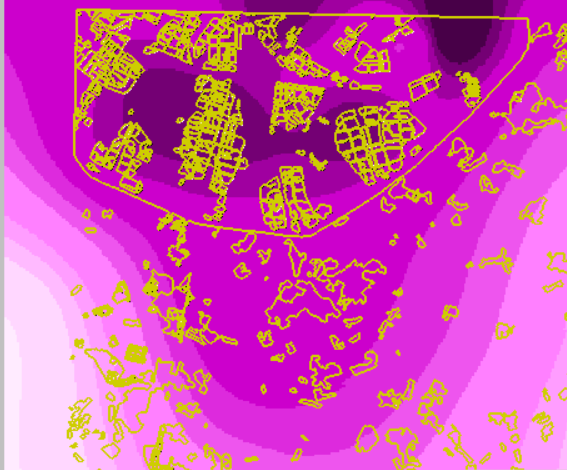
\includegraphics[scale=0.7]{images/111.png}
    \caption{Пример матрицы качеств концентрации выхлопных газов}
    \label{fig:2}
\end{figure}

\section{Классификация цифровых моделей рельефа}
Классифицировать ЦМР можно по нескольким признакам, например по характеру нахождения объектов: регулярные и нерегулярные.

В регулярных ЦМР заметно, что точки моделирующие поверхность земли находятся в пересечении узлов сетки одной дельты, которую проецируют на местность. В подобной сетке форма ячеек может являться различными геометрическими объектами: прямоугольники, квадраты, равносторонние треугольники (рисунок~\ref{fig:3}).

\begin{figure}[h!]
    \center
    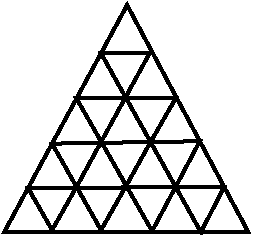
\includegraphics[scale=2]{images/regular.png}
    \caption{Пример регулярной сетки}
    \label{fig:3}
\end{figure}

Такая ЦМР наиболее проста, так как легче провести ее построение, особенно если в районе, в котором строится ЦМР, проводились геодезические работы \cite{9,20}. 

Эффективность достигаемая в условиях однородной местности или городской застройки является достойным преимуществом регулярной ЦМР.

Основными минусами регулярной ЦМР являются:  

\begin{enumerate} 
  \item[1)] ключевые точки рельефа, такие как вершины, впадины, глубины, границы оврагов и т.п., не всегда  совпадают с узлами сетки;
  \item[2)] регулярные ЦМР требуют много трудозатрат при разбиении узловых точек на местности и определении значений высоты в каждой из них;
  \item[3)] при резко меняющемся рельефе, особенно если размеры ячеек очень большие, значительная часть информации может не отразиться в ЦМР (например овраги);
  \item[4)] при слишком маленьких размерах ячеек на достаточно однородной части рельефа, может случиться переизбыток точек, будет занят довольно большой объем памяти и потребуются лишние затраты времени и труда на ввод отметок высоты в узлах сетки \cite{19,22}.
\end{enumerate} 

Регулярные модели нашли применение при проектировани аэродромов, городских улиц, при вертикальной планировке, то есть тогда, когда требуется повышенная детальность исходной информации. 

Также существуют нерегулярные ЦМР, в которых точки размещаются в произвольном порядке, но при этом с заданной частотой и плотностью. Чем сложнее рельеф на местности, тем гуще должна быть построенная сетка (рисунок~\ref{fig:4}). Такая ЦМР позволяет ввести все ключевые точки рельефа~\cite{10}.

Одним из видов нерегулярной сетки является образующаяся при сканировании различных топографических материалов сетка.

У ЦМР, построенной на основе такой сетки, также имеется недостаток -- для каждой точки необходимо вводить ее номер, координаты x, y и отметки высот h.

\begin{figure}[h!]
    \center
    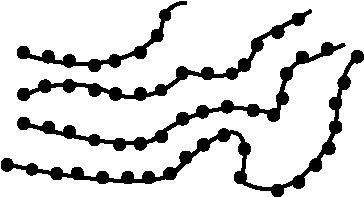
\includegraphics[scale=2.5]{images/unregular.png}
    \caption{Пример нерегулярной сетки}
    \label{fig:4}
\end{figure}

После того как ключевые точки рельефа нерегулярной сетки будут отображены на карту, по данным этих точек будет строиться модель поверхности одним из существующих методов \cite{11,18}. 


